\documentclass{beamer}

\mode<presentation>
{
  \usetheme{Warsaw}
  % or ...

  \setbeamercovered{transparent}
  % or whatever (possibly just delete it)
}

\usepackage{standalone}
\usepackage{tikz}
\usepackage[english]{babel}
% or whatever

\usepackage[utf8]{inputenc}
% or whatever

\usepackage{times}
\usepackage[T1]{fontenc}
% Or whatever. Note that the encoding and the font should match. If T1
% does not look nice, try deleting the line with the fontenc.


\title[Data Sharing and Citations] % (optional, use only with long paper titles)
{Data Sharing and Citations}

\subtitle
{Causal Evidence} % (optional)

\author[Christense, Dafoe, Miguel] % (optional, use only with lots of authors)
{Garre Christensen\inst{1} \and Allan Daffoe\inst{2} \and Edward Miguel\inst{3}}
% - Use the \inst{?} command only if the authors have different
%   affiliation.

\institute[Universities of Somewhere and Elsewhere] % (optional, but mostly needed)
{
  \inst{1}%
  Berkeley Institute for Data Science, UC Berkeley
  \and
  \inst{2}%
  Department of Political Science, Yale University
  \and
  \inst{3}%
  Department of Economics, UC Berkeley}
% - Use the \inst command only if there are several affiliations.
% - Keep it simple, no one is interested in your street address.

\date[Short Occasion] % (optional)
{June 28, 2017 WEAI}

\subject{Talks}
% This is only inserted into the PDF information catalog. Can be left
% out. 



% If you have a file called "university-logo-filename.xxx", where xxx
% is a graphic format that can be processed by latex or pdflatex,
% resp., then you can add a logo as follows:

% \pgfdeclareimage[height=0.5cm]{university-logo}{university-logo-filename}
% \logo{\pgfuseimage{university-logo}}



% Delete this, if you do not want the table of contents to pop up at
% the beginning of each subsection:
%\AtBeginSubsection[]
%{
%  \begin{frame}<beamer>{Outline}
%    \tableofcontents[currentsection,currentsubsection]
%  \end{frame}
%}


% If you wish to uncover everything in a step-wise fashion, uncomment
% the following command: 

%\beamerdefaultoverlayspecification{<+->}


\begin{document}

\begin{frame}
  \titlepage
  \begin{center}
  \begin{large}
  PRELIMINARY--Please do not cite.
  \end{large}
  \end{center}
\end{frame}

\begin{frame}{Outline}
  \tableofcontents
  \begin{center}
  \begin{large}
  PRELIMINARY--Please do not cite.
  \end{large}
  \end{center}
  % You might wish to add the option [pausesections]
\end{frame}


% Since this a solution template for a generic talk, very little can
% be said about how it should be structured. However, the talk length
% of between 15min and 45min and the theme suggest that you stick to
% the following rules:  

% - Exactly two or three sections (other than the summary).
% - At *most* three subsections per section.
% - Talk about 30s to 2min per frame. So there should be between about
%   15 and 30 frames, all told.

\section{Introduction}

\begin{frame}{Data Sharing Incentives}{}
  % - A title should summarize the slide in an understandable fashion
  %   for anyone how does not follow everything on the slide itself.

  \begin{itemize}
  \item
    Shared data is a public good. (See Newton 1675)
  \item
    Public goods are often undersupplied.
  \item 
  	 Is there private incentive?
  	 \begin{itemize}
  	 \item Citations
  	 \item Promotion \& tenure
  	 \end{itemize} 
  \end{itemize}
\end{frame}

\begin{frame}{Existing Evidence}
\begin{itemize}
\item \href{http://journals.plos.org/plosone/article?id=10.1371/journal.pone.0000308}{Piwowar, Day, Fridsma (2007)}: 69\% more citations for cancer microarray clinical trials papers (N=85).
\item \href{https://peerj.com/articles/175/}{Piwowar, Vision (2013)}: 9\% more citations for gene expression microarray papers with public data (N=10,555).
\item \textit{Journal of Peace Research}
\begin{itemize}
\item
Yes: Gleditsch, Metelits, Strand. 2003. ``Posting Your Data: Will You Be Scooped or Will You Be Famous?''
\item No: \href{http://journals.sagepub.com/doi/abs/10.1177/0049124107306664}{Abbott 2007}
\item Yes: Strand, Nordkvelle, Gleditsch. 2014. ``Posting Your Data: Will You Remain Famous?''

\end{itemize}
\end{itemize}
\end{frame}


{ % all template changes are local to this group.
    \setbeamertemplate{navigation symbols}{}
    \begin{frame}[plain]
        \begin{tikzpicture}[remember picture,overlay]
            \node[at=(current page.center)] {
                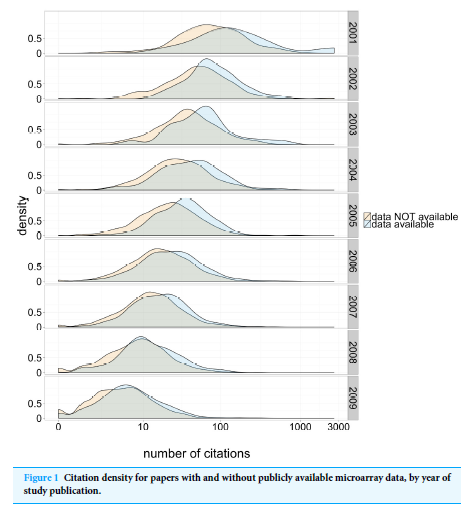
\includegraphics[height=\paperheight]{../images/peerj_piwowar_vision2013.PNG}
            };
        \end{tikzpicture}
     \end{frame}
}
{ % all template changes are local to this group.
    \setbeamertemplate{navigation symbols}{}
    \begin{frame}[plain]
        \begin{tikzpicture}[remember picture,overlay]
            \node[at=(current page.center)] {
                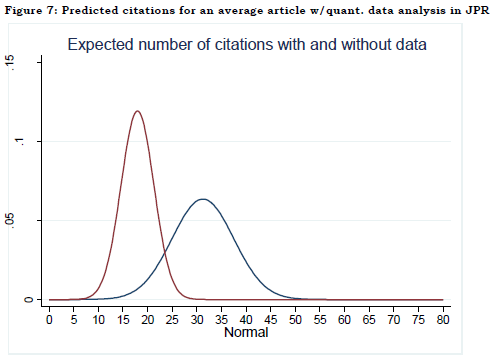
\includegraphics[width=\paperwidth]{../images/jpr.PNG}
            };
        \end{tikzpicture}
     \end{frame}
}

\begin{frame}{The Case of Political Science}
Exploit plausibly exogenous variation in data availability caused by the abrupt change in editorial policy at a top political science journal, \textit{The American Journal of Political Science} (\textit{AJPS}). 

Rick Wilson became the editor on January 1, 2010:
\begin{quote} ``If a manuscript is accepted for publication it will not be published unless the first footnote explicitly notes where the data used in the study can be obtained for purposes of replication and should note any sources that funded the research.''
\end{quote}
\end{frame}

\begin{frame}{The Case of Political Science}
The first issue Wilson edited was published in October 2010. After discussion with the board members in April of 2012, the policy was expanded to require posting data in the journal's public archive at \href{https://thedata.harvard.edu/dvn/dv/ajps}{Harvard's Dataverse} and Wilson strengthened his enforcement of this policy. This policy was printed in the July 2012 issue, and was enforced thereafter.
\vspace{0.25in}

There was no policy change at the other top political science journal, \textit{American Political Science Review}, (\textit{APSR}).
\end{frame}


\begin{frame}{Pre-Analysis Plan}

\begin{itemize}
\item Short pre-analysis plan before data collection.
\item Available at \url{https://osf.io/qxpr6/}
\end{itemize}

\begin{align}\label{firststage} 
availability_i &= \alpha_1 +\beta_1 AJPS_i + \beta_2 Post2010_i + \beta_3 Post2012_i \\ \notag
& + {\color{red} \beta_4 AJPS*Post2010_i + \beta_5 AJPS*Post2012_i } \\
& + g_1(Time) + h_1(Year) +\nu_i \notag
\end{align}

\begin{align}
citations_i &=\alpha_2 +\eta_1 AJPS_i + \eta_2 Post2010_i+ \eta_3 Post2012_i \\ 
& + \eta_4 \hat{availability_i}+g_2(Time) + h_2(Year) +u_i \notag
\end{align}

\end{frame}
\begin{frame}{Summary Statistics}
\begin{itemize}
\item Citations highly concentrated.
\item Citations increase over time.
\item Citations affected by journal policy.
\end{itemize}
\end{frame}

{ % all template changes are local to this group.
    \setbeamertemplate{navigation symbols}{}
    \begin{frame}[plain]
        \begin{tikzpicture}[remember picture,overlay]
            \node[at=(current page.center)] {
                \includegraphics[width=\paperwidth]{../output/cite_histo.png}

            };
        \end{tikzpicture}
     \end{frame}
     
     \begin{frame}[plain]
        \begin{tikzpicture}[remember picture,overlay]
            \node[at=(current page.center)] {
                \includegraphics[width=\paperwidth]{../output/cite_time.png}

            };
        \end{tikzpicture}
     \end{frame}
    
    \begin{frame}[plain]
        \begin{tikzpicture}[remember picture,overlay]
            \node[at=(current page.center)] {
                \includegraphics[width=\paperwidth]{../output/avail_time.png}
            };
        \end{tikzpicture}
     \end{frame}
}


\section{Results}
\begin{frame}
\begin{itemize}
\item Naive OLS results
\item First stage
\item 2SLS
\item Exclusion Restriction
\end{itemize}
\end{frame}

\begin{frame}{}
\scalebox{0.75}{\input{../output/naive.tex}}
\end{frame}

\begin{frame}{}
\scalebox{0.9}{\input{../output/naive-simp.tex}}
\end{frame}

%\begin{frame}{}
%\scalebox{0.75}{\input{../output/naiveLN.tex}}
%\end{frame}

\begin{frame}{}
\scalebox{0.83}{\input{../output/naiveLN-simp.tex}}
\end{frame}

\begin{frame}{}
\scalebox{0.50}{\input{../output/first.tex}}
\end{frame}

\begin{frame}{}
\scalebox{0.70}{\input{../output/ivreg-simp.tex}}
\end{frame}

\begin{frame}{}
\scalebox{0.70}{\input{../output/ivregLN-simp.tex}}
\end{frame}

{ % all template changes are local to this group.
    \setbeamertemplate{navigation symbols}{}
    \begin{frame}[plain]
        \begin{tikzpicture}[remember picture,overlay]
            \node[at=(current page.center)] {
                \includegraphics[width=\paperwidth]{../output/topicXjournalXpost2010.png}
            };
        \end{tikzpicture}
     \end{frame}
}


{ % all template changes are local to this group.
    \setbeamertemplate{navigation symbols}{}
    \begin{frame}[plain]
        \begin{tikzpicture}[remember picture,overlay]
            \node[at=(current page.center)] {
                \includegraphics[width=\paperwidth]{../output/topicXjournalXpost2012.png}
            };
        \end{tikzpicture}
     \end{frame}
}

{ % all template changes are local to this group.
    \setbeamertemplate{navigation symbols}{}
    \begin{frame}[plain]
        \begin{tikzpicture}[remember picture,overlay]
            \node[at=(current page.center)] {
                \includegraphics[width=\paperwidth]{../output/typeXjournalXpost2010.png}
            };
        \end{tikzpicture}
     \end{frame}
}

{ % all template changes are local to this group.
    \setbeamertemplate{navigation symbols}{}
    \begin{frame}[plain]
        \begin{tikzpicture}[remember picture,overlay]
            \node[at=(current page.center)] {
                \includegraphics[width=\paperwidth]{../output/typeXjournalXpost2012.png}
            };
        \end{tikzpicture}
     \end{frame}
}

{ % all template changes are local to this group.
    \setbeamertemplate{navigation symbols}{}
    \begin{frame}[plain]
        \begin{tikzpicture}[remember picture,overlay]
            \node[at=(current page.center)] {
                \includegraphics[width=\paperwidth]{../output/rankXjournalXpost2010.png}
            };
        \end{tikzpicture}
     \end{frame}
}

{ % all template changes are local to this group.
    \setbeamertemplate{navigation symbols}{}
    \begin{frame}[plain]
        \begin{tikzpicture}[remember picture,overlay]
            \node[at=(current page.center)] {
                \includegraphics[width=\paperwidth]{../output/rankXjournalXpost2012.png}
            };
        \end{tikzpicture}
     \end{frame}
}

\begin{frame}{}
\scalebox{0.60}{\input{../output/exclusion.tex}}
\end{frame}

\section{Conclusion}

\begin{frame}{Preliminary Conclusions}

  % Keep the summary *very short*.
  \begin{itemize}
  \item
    Top political science papers with public data are cited more.
  \item
    Some suggestive, not strong, evidence of causality.
  \item
    Journal policy does not appear to have changed submissions.
    \begin{itemize}
    \item IV identification strategy OK.
    \end{itemize}
  \end{itemize}
\end{frame}

\begin{frame}{Future}
	\begin{itemize}
	\item Data quality checks.
	\item Economics: AER \& QJE 2001-2009
	\end{itemize}
\end{frame}

\end{document}


